\documentclass{abntex2}
\usepackage[utf8]{inputenc}
\usepackage{graphicx}
\usepackage[num]{abntex2cite}

\titulo{Experimento 3: Modelamento elétrico simplificado do sistema cardiovascular}
\autor{Lucas Rezende de Macedo - 14/0026363\\Jônatas Ribeiro Senna Pires - 14/0090983}
\data{29 de Abril de 2018}
\local{Brasília, Distrito Federal}

\begin{document}

\imprimircapa
\imprimirfolhaderosto

\tableofcontents
\listoffigures
\clearpage

\chapter{Experiências}

O procedimento experimental consiste na simulação de um circuito que modela, de forma simplificada, o sistema cardiovascular. O circuito simulado pode ser observado na
imagem \ref{fig:circuitop}

\begin{figure}[h]
  \centering
  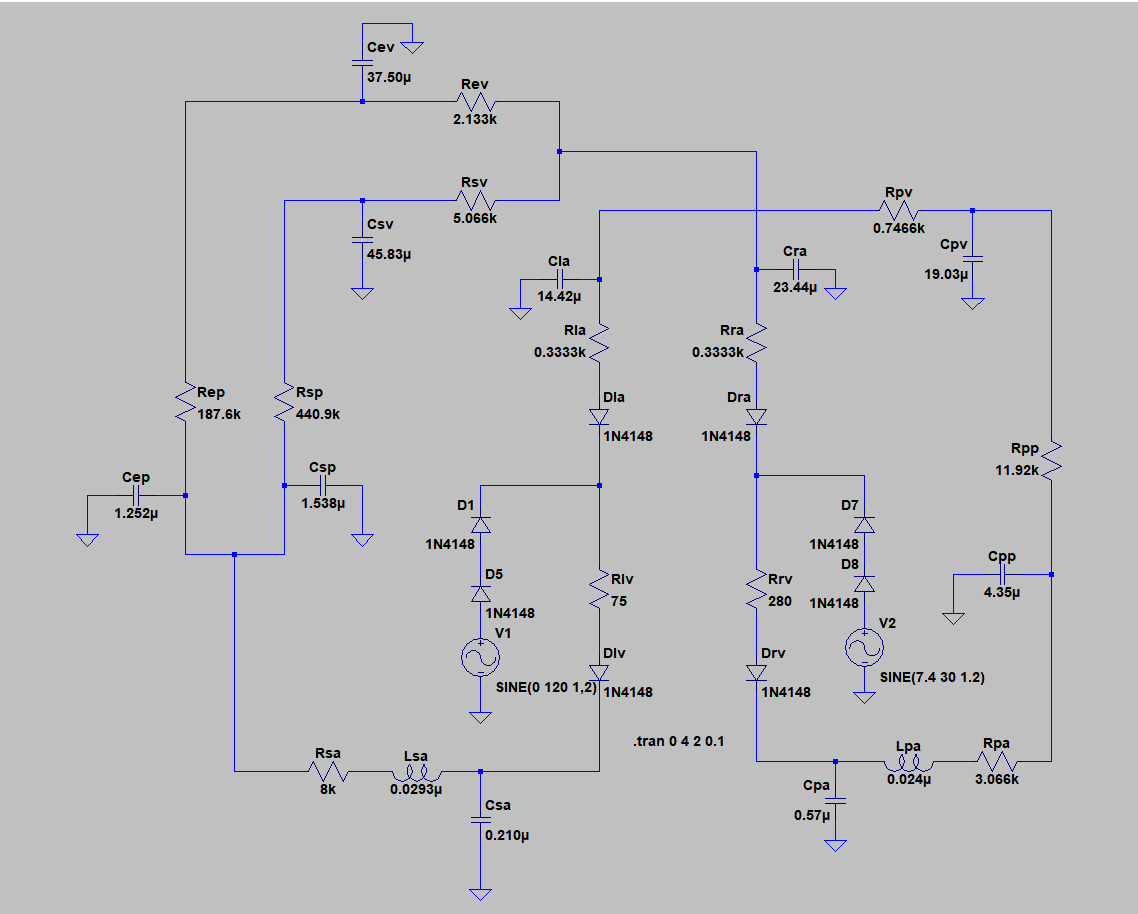
\includegraphics[scale = 0.5]{circuitop.png}
  \caption{Circuito que modela o sistema cardiovascular simulado no procedimento experimental.}
  \label{fig:circuitop}
\end{figure}


\section{Experiência}

Foi escolhido o simulador LTSpice para a realização do experimento. Após a montagem do esquemático no programa (de acordo com a figura \ref{fig:circuitop}).
\\Foram coletadas as curvas de tensão do sinal referente a pressão na entrada da artéria aorta (saída do ventrículo esquerdo) com o offset de 7,4V na fonte de tensão 2 sugerido pelo artigo lido, como mostra a figura \ref{fig:aorta1}.
\pagebreak
\begin{figure}[h]
  \centering
  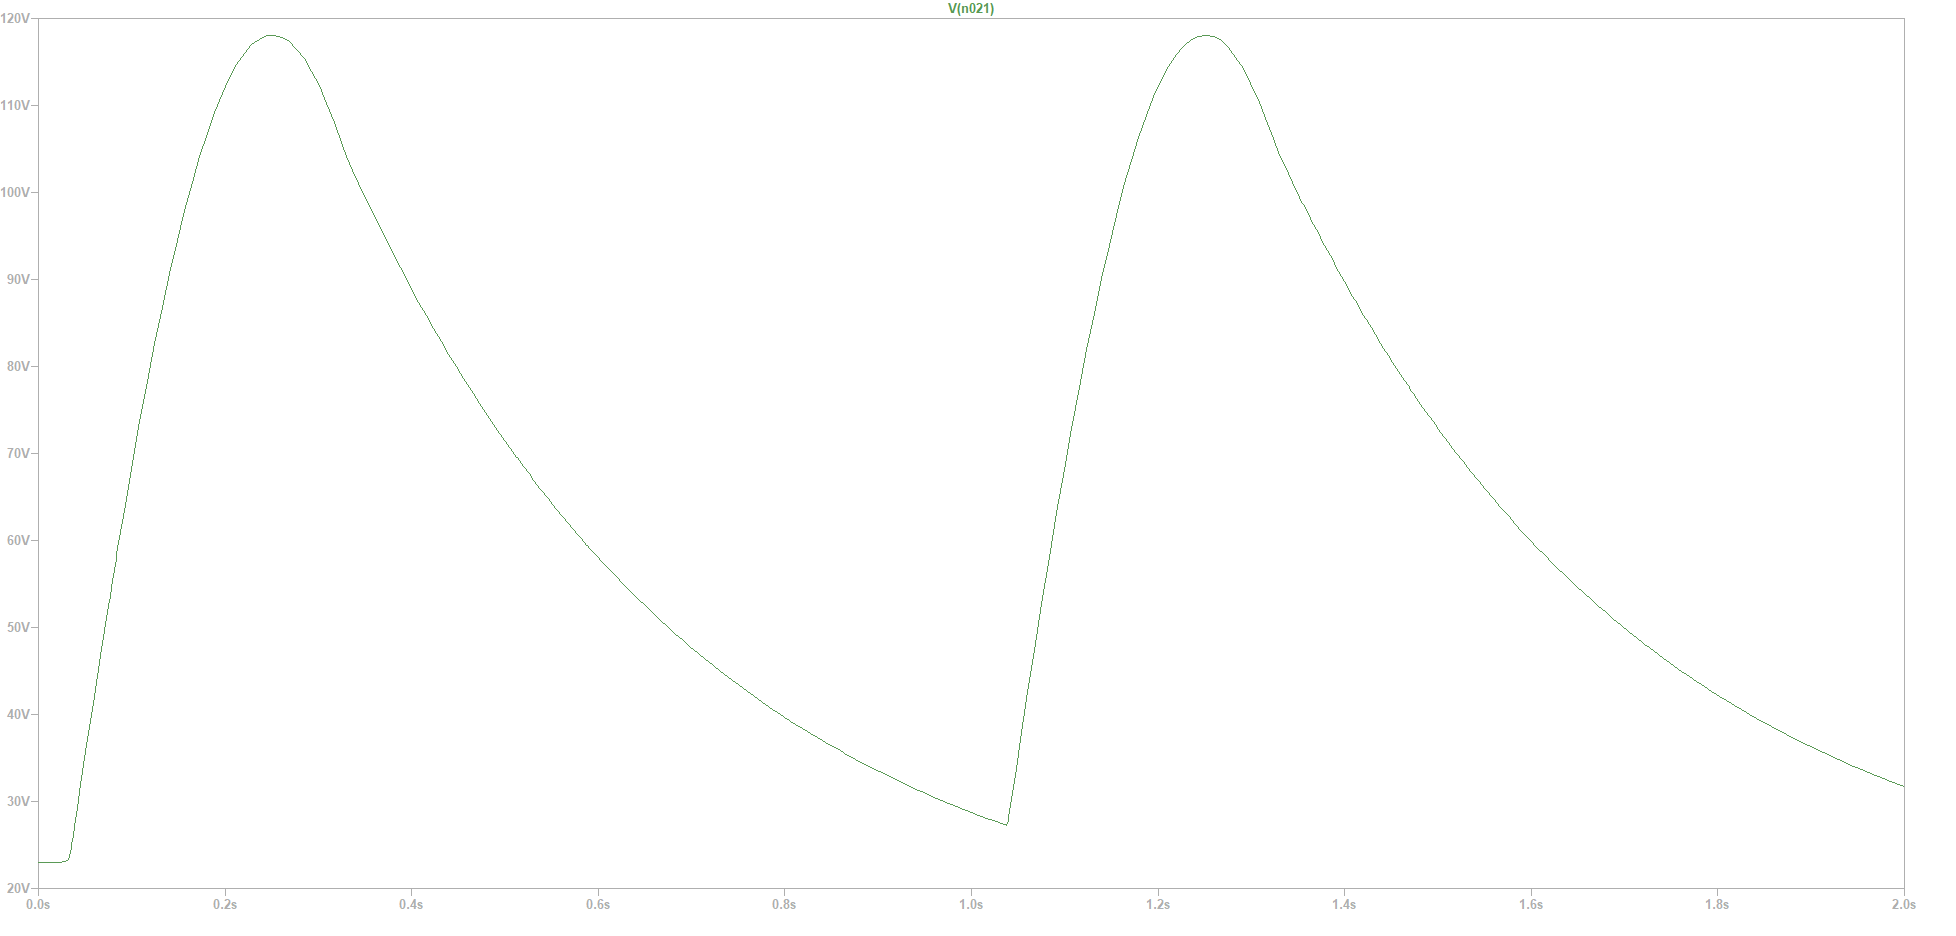
\includegraphics[scale = 0.3]{aorta_v10_v274.png}
  \caption{Gráfico da tensão referente à pressão arterial na entrada da artéria aorta com offset de 7,4V na fonte 2}
  \label{fig:aorta1}
\end{figure}

\\Foram coletadas as curvas de tensão do sinal referente a pressão na entrada da artéria pulmonar (saída do ventrículo direito) com o offset de 7,4V na fonte de tensão 2 sugerido pelo artigo lido, como mostra a figura \ref{fig:pulmonar1}.

\begin{figure}[h]
  \centering
  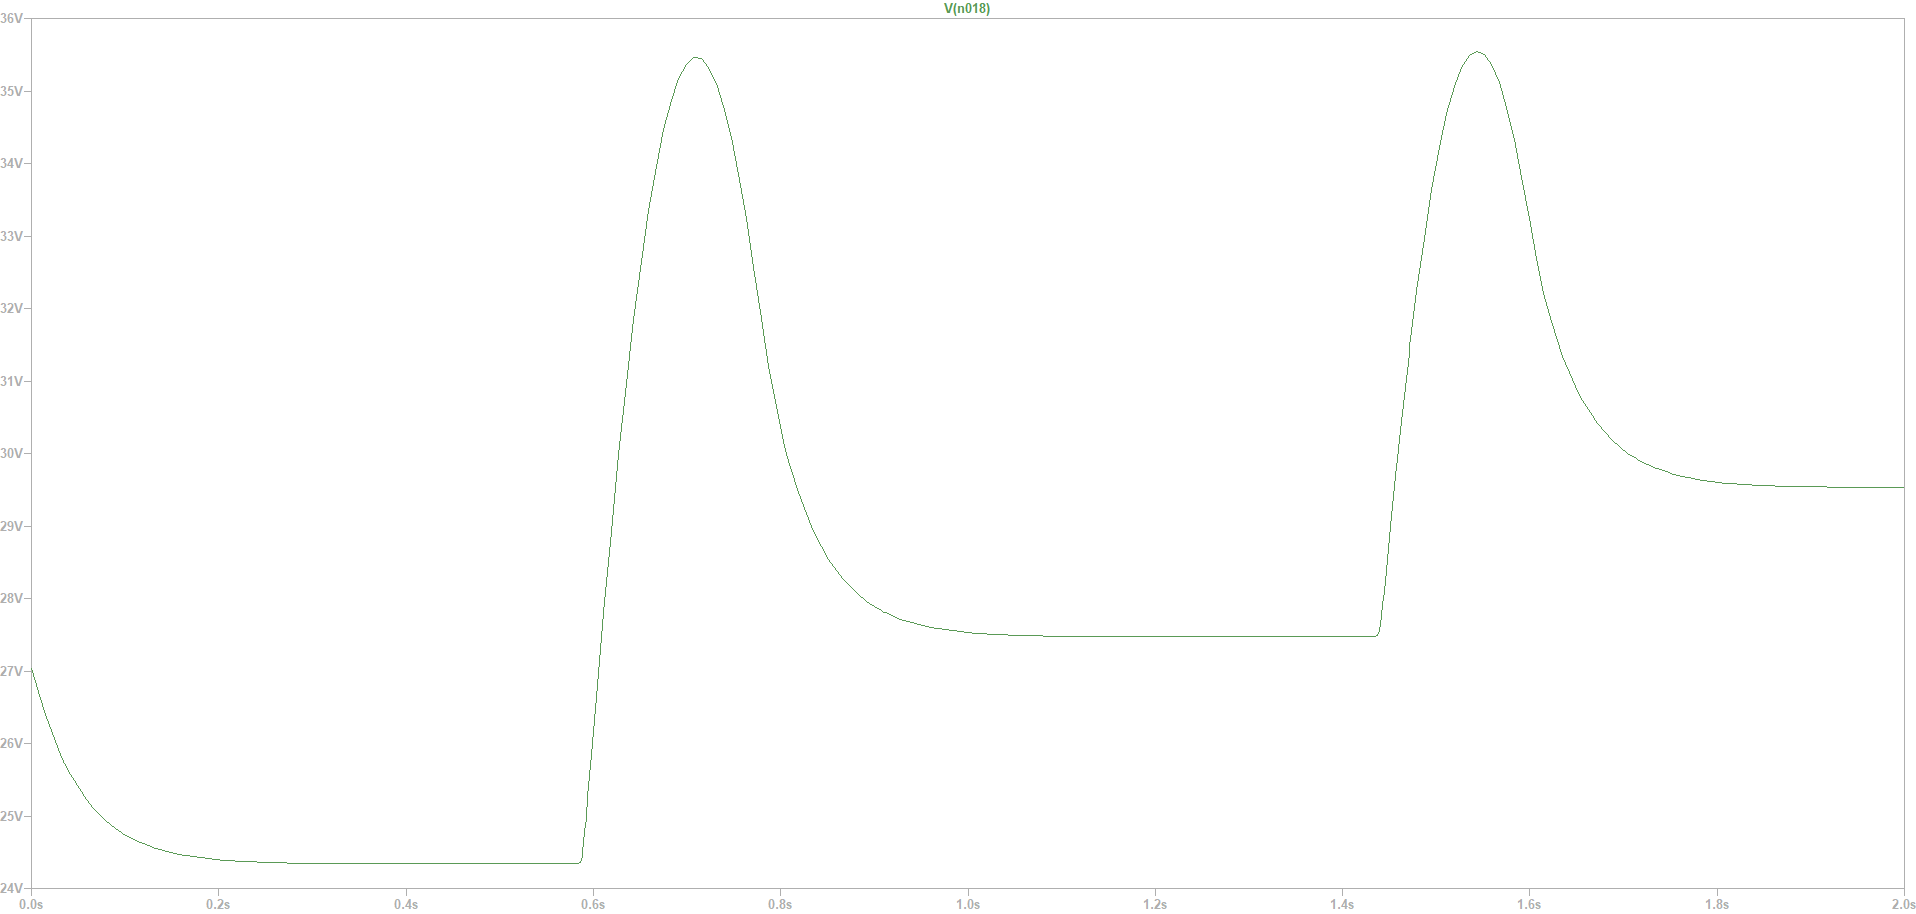
\includegraphics[scale = 0.3]{pulmonar_v10_v274.png}
  \caption{Gráfico da tensão referente à pressão arterial na entrada da artéria pulmonar com offset de 7,4V na fonte 2}
  \label{fig:pulmonar1}
\end{figure}

\\Foram coletadas as curvas de tensão do sinal referente a pressão na entrada do ventrículo esquerdo, com o offset de 7,4V na fonte de tensão 2 sugerido pelo artigo lido, como mostra a figura \ref{fig:ventriculo1}.

\begin{figure}[h]
  \centering
  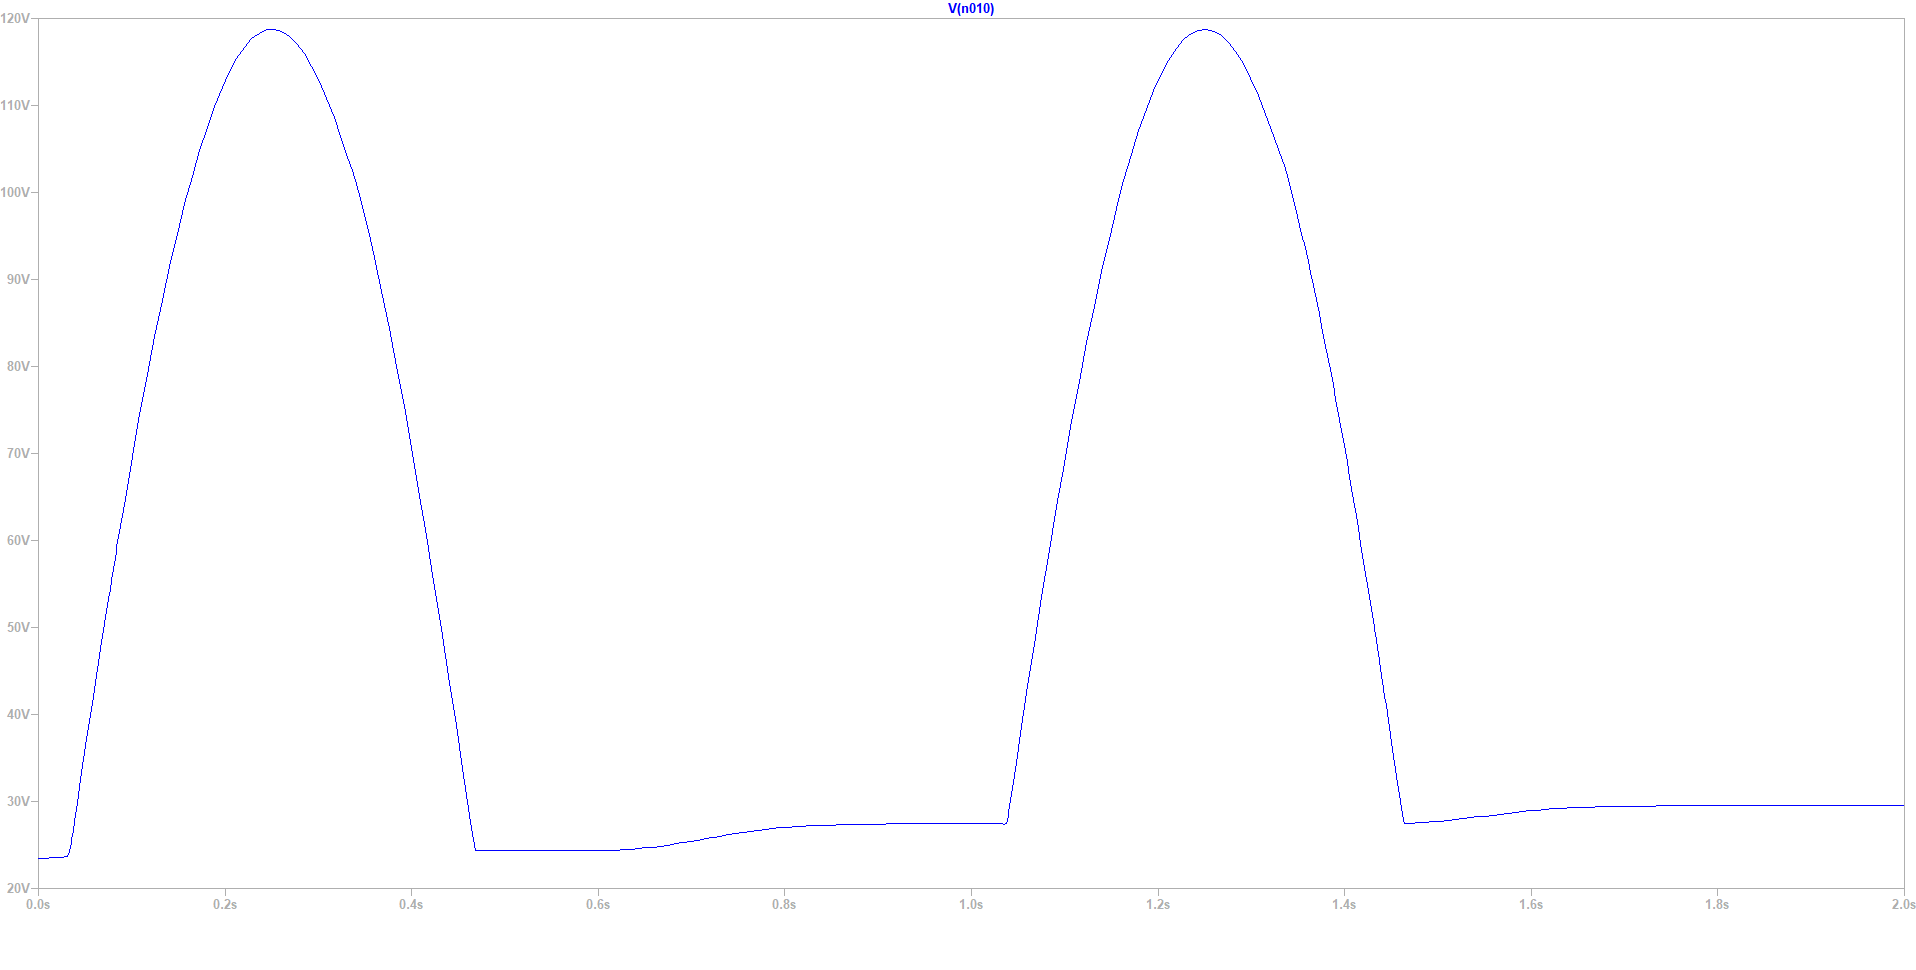
\includegraphics[scale = 0.3]{ventriculo_esq_v10_v274.png}
  \caption{Gráfico da tensão referente à pressão arterial na entrada do ventrículo esquerdo com offset de 7,4V na fonte 2}
  \label{fig:ventriculo1}
\end{figure}
\pagebreak
\\\\Para efeitos de comparação, também foram coletados os dados nos mesmos pontos, mas com diferentes offsets nas fontes, assim como indicados nas figuras de \ref{fig:aorta2} e \ref{fig:ventriculo3}
\\Curvas de tensão do sinal referente a pressão na entrada da artéria aorta (saída do ventrículo esquerdo) com nenhum offset aplicado em ambas as fontes, como mostra a figura \ref{fig:aorta2}.

\begin{figure}[h]
  \centering
  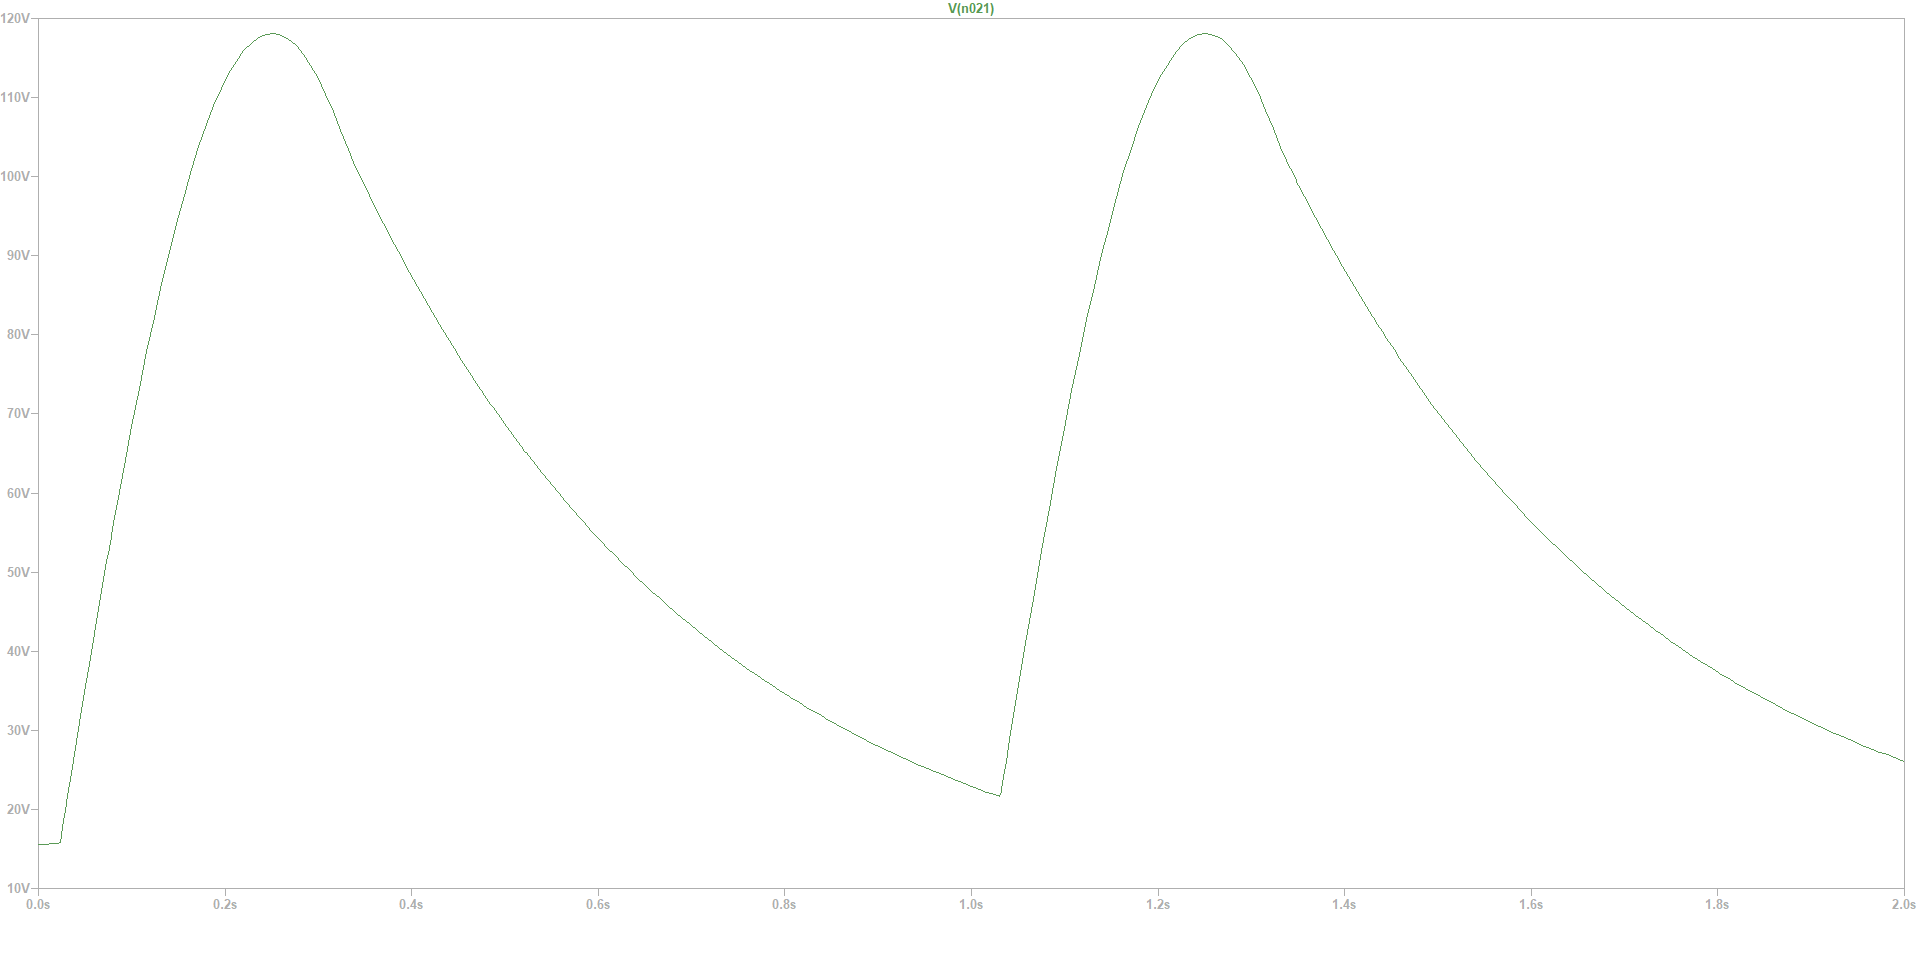
\includegraphics[scale = 0.3]{aorta_v10_v20.png}
  \caption{Gráfico da tensão referente à pressão arterial na entrada da artéria aorta sem offset em ambas as fontes}
  \label{fig:aorta2}
\end{figure}

\\Curvas de tensão do sinal referente a pressão na entrada da artéria pulmonar (saída do ventrículo direito) com nenhum offset aplicado em ambas as fontes, como mostra a figura \ref{fig:pulmonar2}.

\begin{figure}[h]
  \centering
  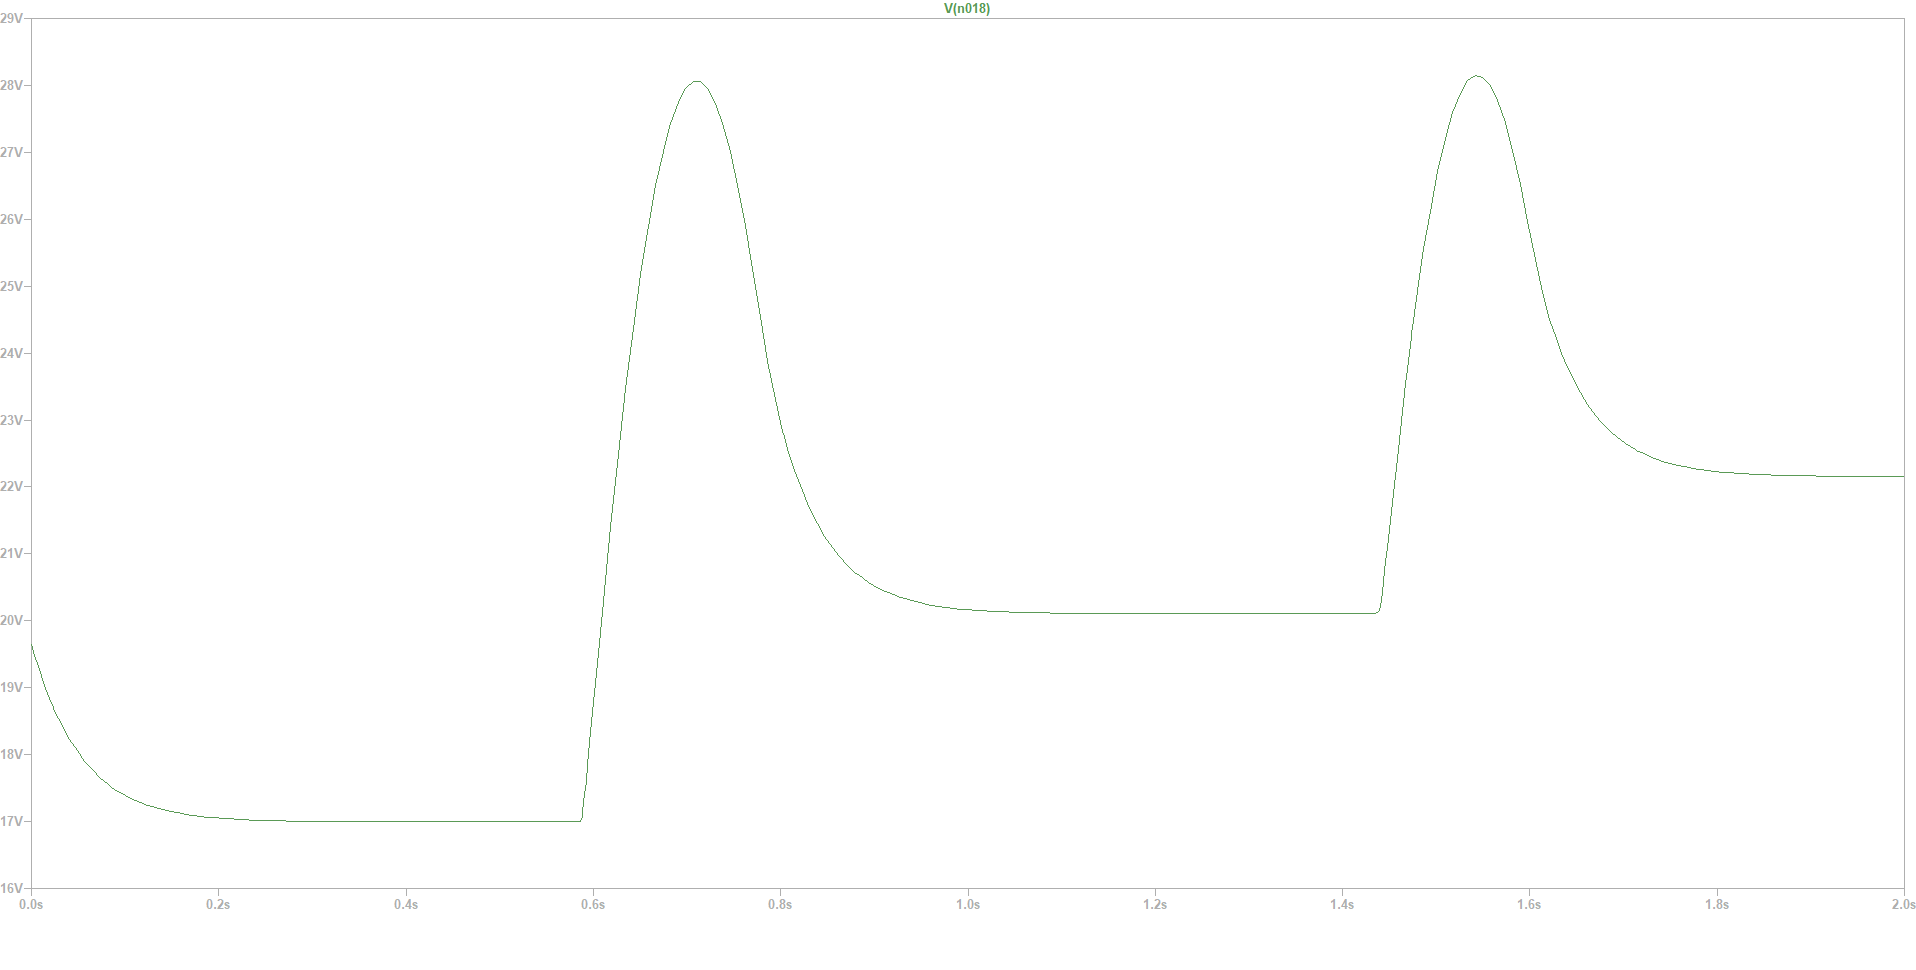
\includegraphics[scale = 0.3]{pulmonar_v10_v20.png}
  \caption{Gráfico da tensão referente à pressão arterial na entrada da artéria pulmonar sem offset em ambas as fontes}
  \label{fig:pulmonar2}
\end{figure}
\pagebreak

\\Curvas de tensão do sinal referente a pressão na entrada do ventrículo esquerdo, com nenhum offset aplicado em ambas as fontes, como mostra a figura \ref{fig:ventriculo2}.

\begin{figure}[h]
  \centering
  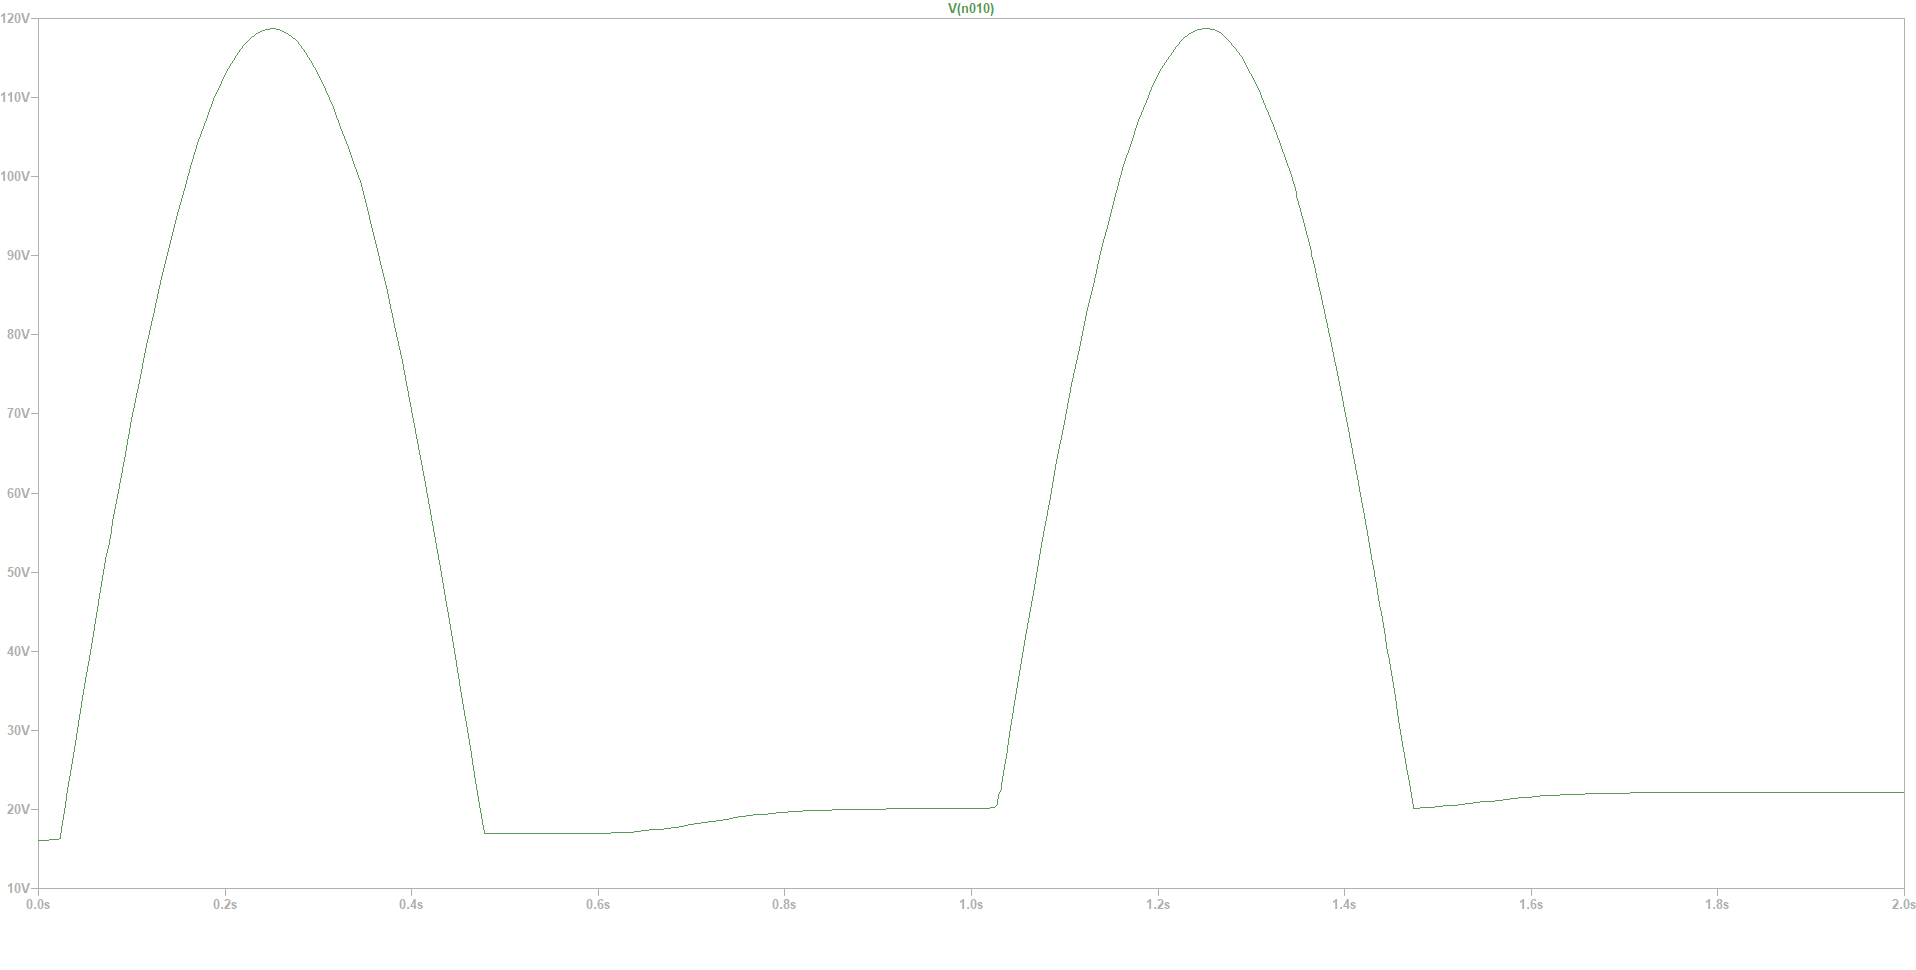
\includegraphics[scale = 0.3]{ventriculo_esq_v10_v20.png}
  \caption{Gráfico da tensão referente à pressão arterial na entrada do ventrículo esquerdo sem offset em ambas as fontes}
  \label{fig:ventriculo2}
\end{figure}

\\Curvas de tensão do sinal referente a pressão na entrada da artéria aorta (saída do ventrículo esquerdo) com offset de 7,4V aplicado em ambas as fontes, como mostra a figura \ref{fig:aorta3}.
\pagebreak
\begin{figure}[h]
  \centering
  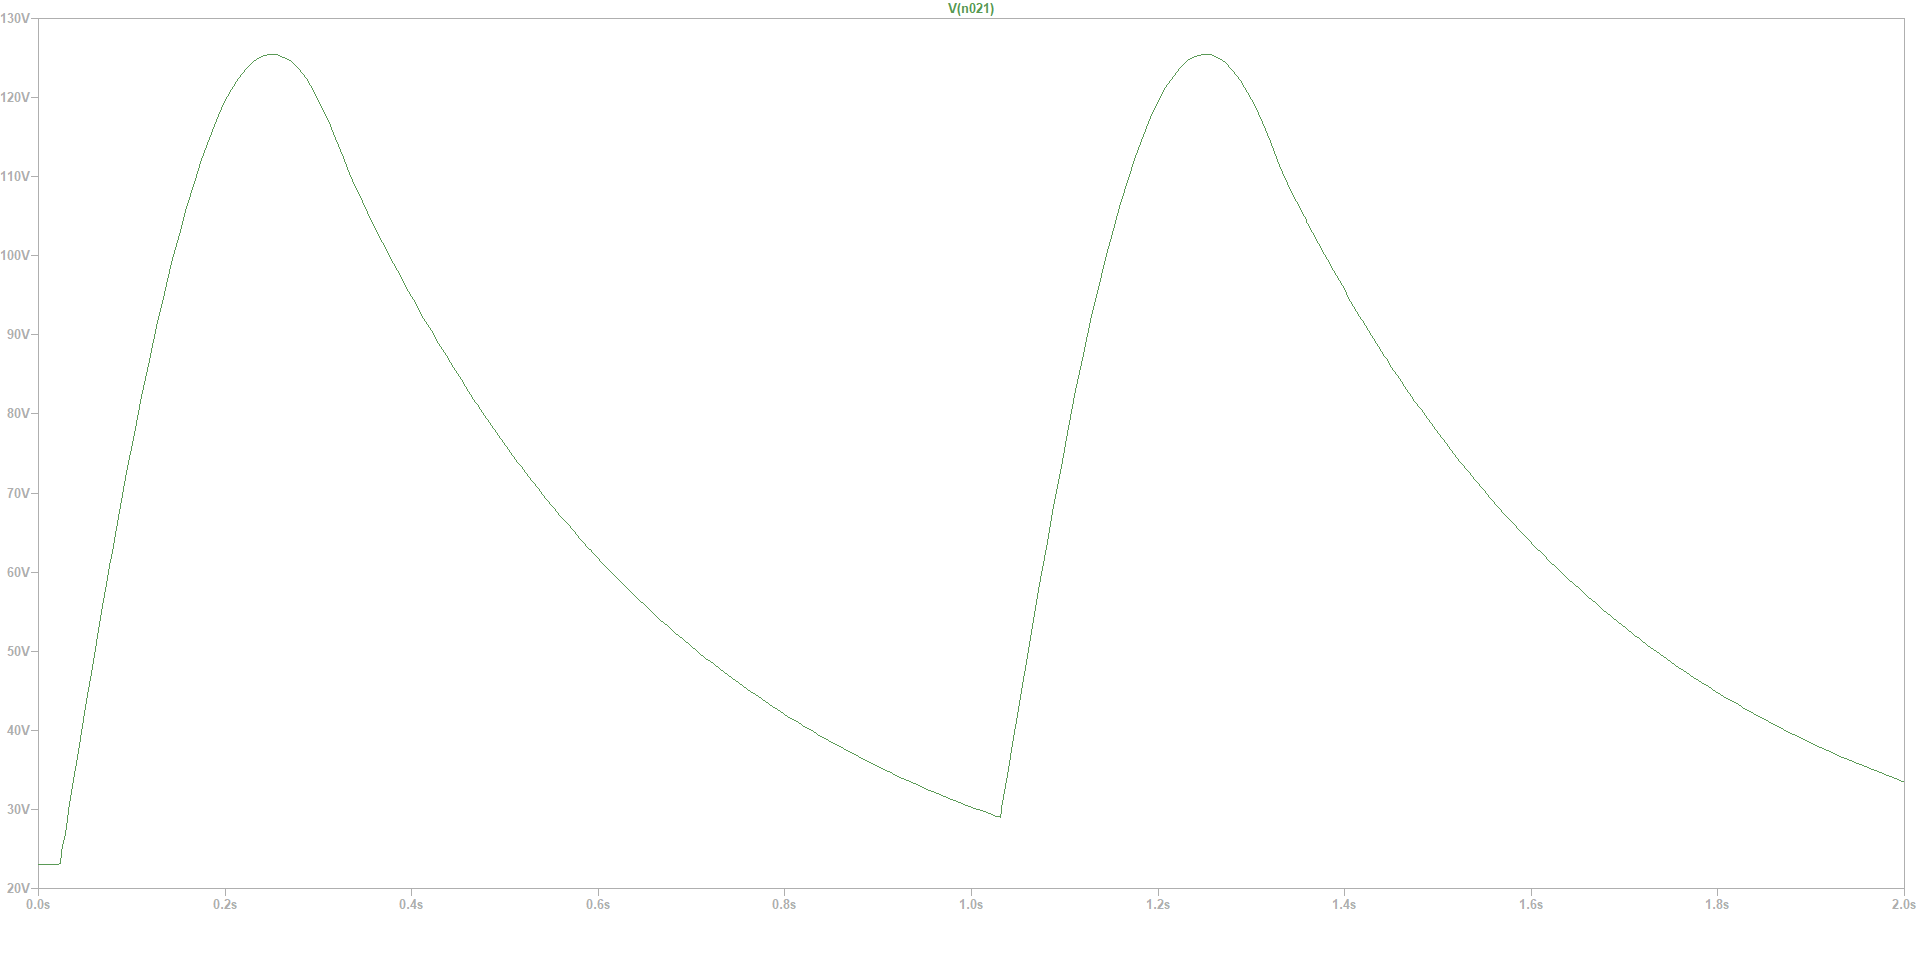
\includegraphics[scale = 0.3]{aorta_v174_v274.png}
  \caption{Gráfico da tensão referente à pressão arterial na entrada da artéria aorta com offset de 7,4V em ambas as fontes}
  \label{fig:aorta3}
\end{figure}

\\Curvas de tensão do sinal referente a pressão na entrada da artéria pulmonar (saída do ventrículo direito) com offset de 7,4V aplicado em ambas as fontes, como mostra a figura \ref{fig:pulmonar3}.

\begin{figure}[h]
  \centering
  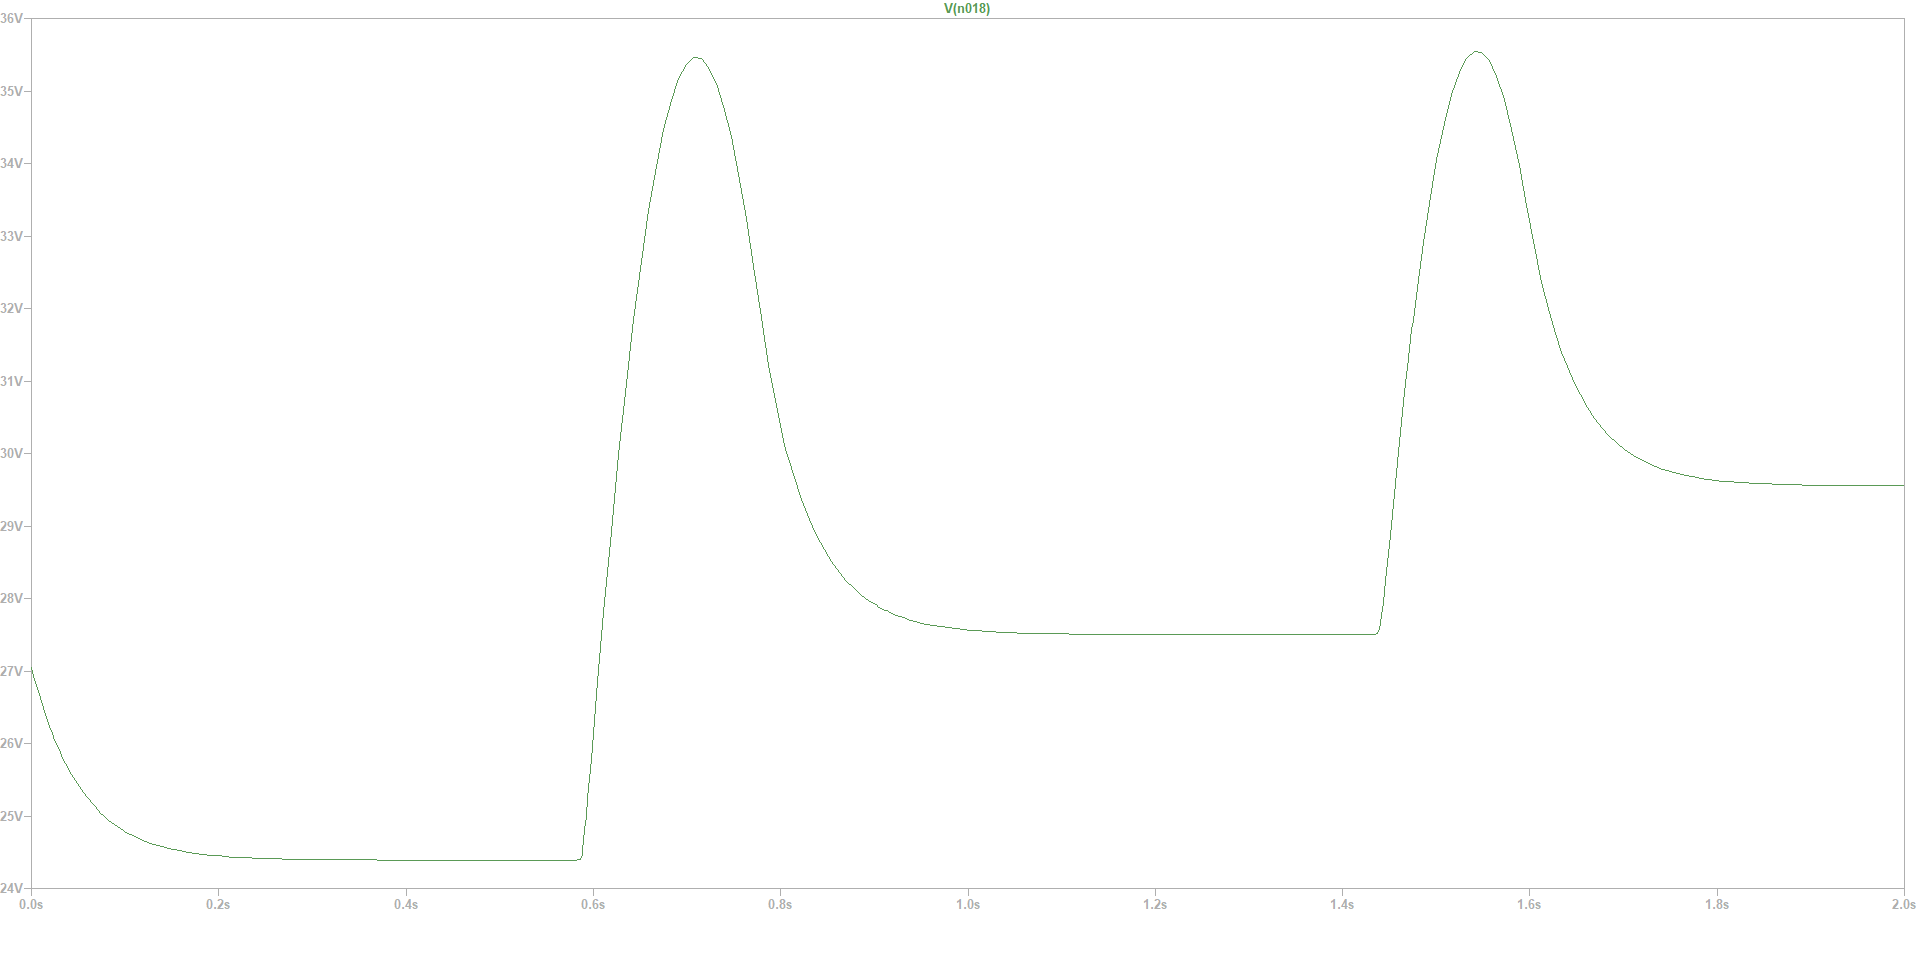
\includegraphics[scale = 0.3]{pulmonar_v174_v274.png}
  \caption{Gráfico da tensão referente à pressão arterial na entrada da artéria pulmonar com offset de 7,4V em ambas as fontes}
  \label{fig:pulmonar3}
\end{figure}
\pagebreak
Curvas de tensão do sinal referente a pressão na entrada do ventrículo esquerdo, com offset de 7,4V aplicado em ambas as fontes, como mostra a figura \ref{fig:ventriculo3}.

\begin{figure}[h]
  \centering
  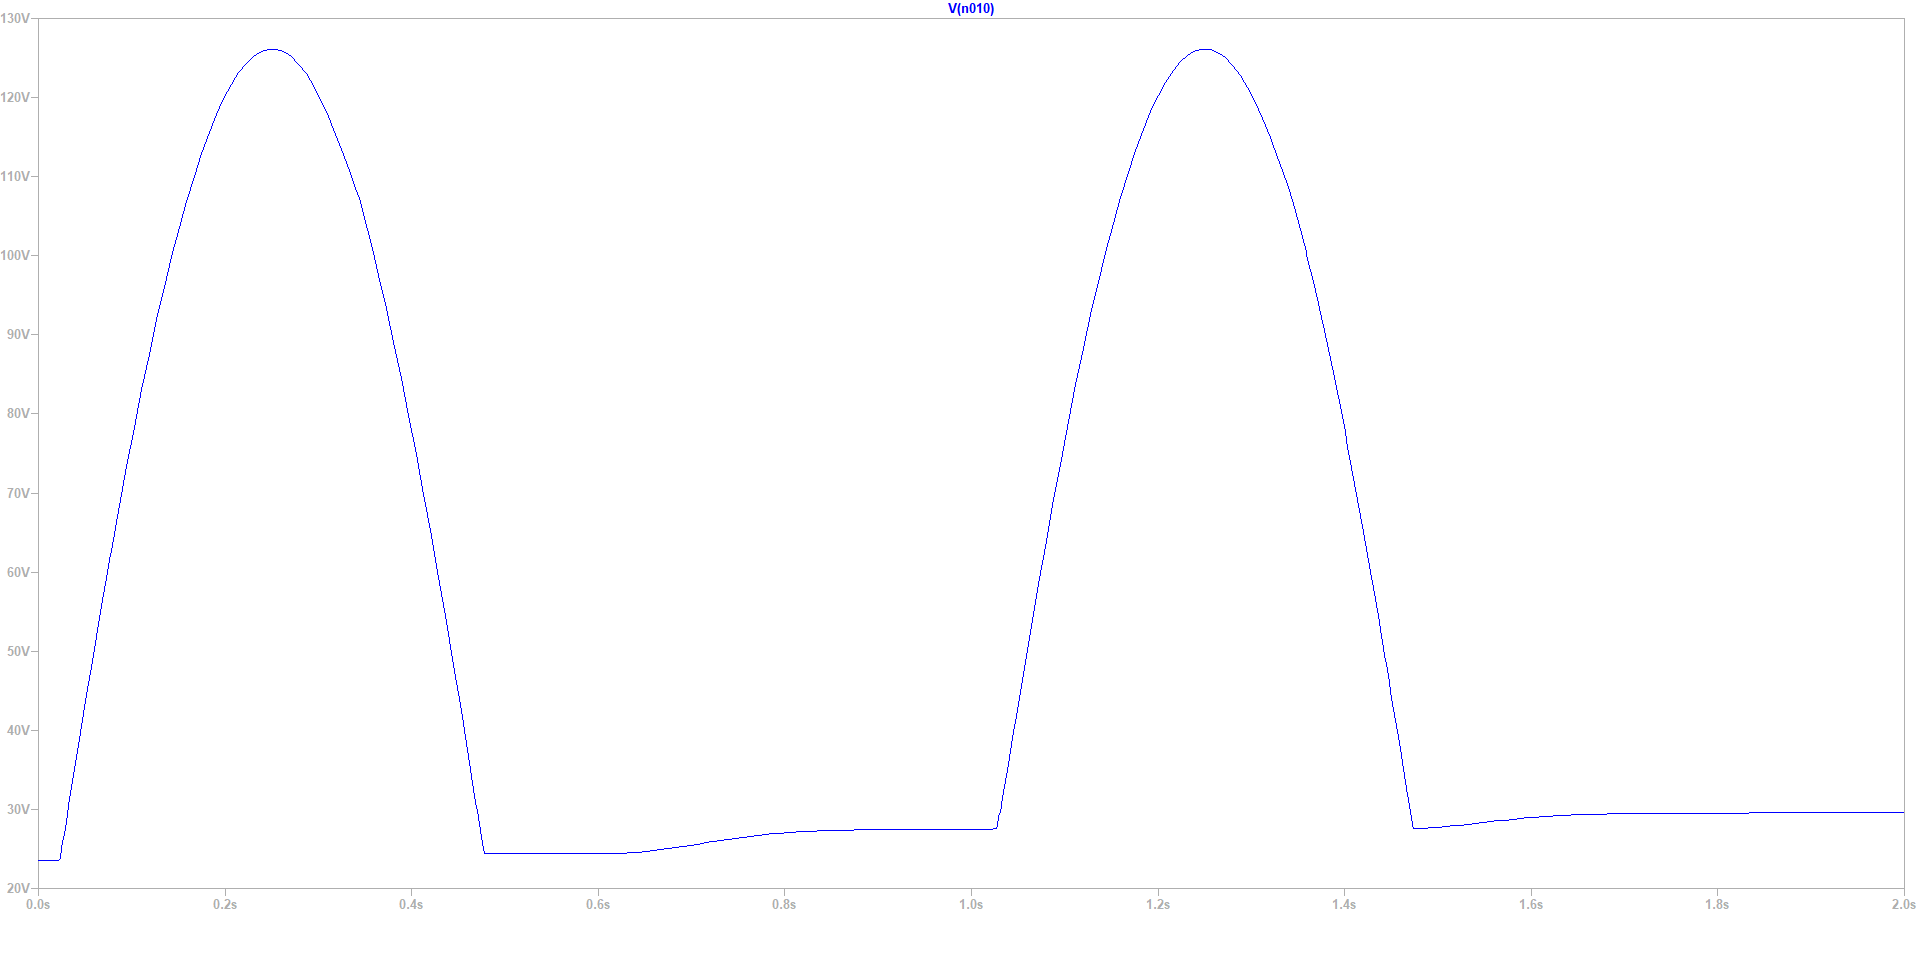
\includegraphics[scale = 0.3]{ventriculo_esq_v174_v274.png}
  \caption{Gráfico da tensão referente à pressão arterial na entrada do ventrículo esquerdo com offset de 7,4V em ambas as fontes}
  \label{fig:ventriculo3}
\end{figure}

\chapter{Discussão}

\section{Questão 1 - Comparação entre gráficos simulados e esperados}

Podemos observar pela figura \ref{fig:aorta1} que a curva de entrada da artéria aorta possui formato semelhante apesar de ser mais suave que a obtida no artigo[4], devido ao modelo utilizado por nós ser mais simplificado que o modelo utilizado no artigo.

A curva de entrada da artéria pulmonar obtida na simulação (figura \ref{fig:pulmonar1}) é diferente da curva do artigo, provavelmente devido às simplificações feitas no circuito simulado.

A curva de entrada do ventriculo esquerdo simulada (figura \ref{fig:ventriculo1}) é bastante semelhante à curva obtida no artigo, devidao ao fate de essa parte do circuito ser a parte na qual foram realizadas menos simplificações.

\section{Questão 2 - Quais as grandezas elétricas equivalentes às grandezas de pressão arterial, fluxo sanguíneo, volume, resistência e complacência no sistema cardiovascular?}

As grandezas elétricas equivalentes ãs grandezas de pressão arterial, fluxo sanguíneo, volume, resistencia e complacência são as seguintes:

\begin{itemize}
  \item {Pressão arterial: Voltagem}
  \item {Fluxo sanguíneo: Corrente életrica}
  \item {Volume: Carga életrica}
  \item {Resistência: Resistência}
  \item {Complacência: Capacitância}
\end{itemize}

\section{Questão 3 - Relação entre as válvulas e os diodos}

Tomando como base a figura \ref{fig:coracao}, é possível afirmar que as válvulas se referenciam aos seguintes diodos:
\begin{itemize}
  \item {Válvula 1 - diodo DRA}
  \item {Válvula 2 - diodo DRV}
  \item {Válvula 3 - diodo DLA}
  \item {Válvula 4 - diodo DLV}
\end{itemize}

\begin{figure}[h]
  \centering
  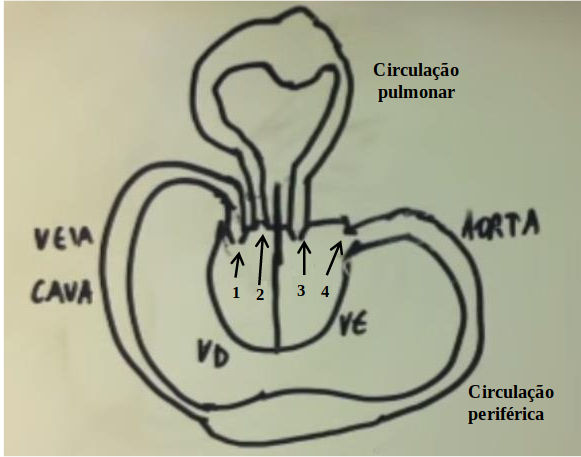
\includegraphics[scale = 0.4]{coracao.png}
  \caption{Modelo do coração como duas bombas hidráulicas; Válvulas representadas de 1 a 4.}
  \label{fig:coracao}
\end{figure}
\pagebreak

\section{Questão 4 - Significado das abreviaturas}

Os significados das siglas dos compartimentos utilizados e os componentes do circuito que os representam são os seguintes:

\begin{itemize}
  \item {ev: sistema venoso extra-esplâncnico (\emph{extrasplanchnic venous}) - $R_{ev}$, $C_{ev}$}
  \item {ep: sistema periférico extra-esplâncnico (\emph{extrasplanchnic peripheral}) - $R_{ep}$, $C_{ep}$}
  \item {sv: sistema venoso esplâncnico (\emph{splanchnic venous}) - $R_{sv}$, $C_{sv}$}
  \item {sp: sistema periférico esplâncnico (\emph{splanchnic peripheral}) - $R_{sp}$, $C_{sp}$}
  \item {pv: sistema venoso pulmonar (\emph{pulmonary venous}) - $R_{pv}$, $C_{pv}$}
  \item {pp: sistema periférico pulmonar (\emph{pulmonary peripheral}) - $R_{pp}$, $C_{pp}$}
  \item {pa: sistema arterial pulmonar (\emph{pulmonary arterial}) - $L_{pa}$, $R_{pa}$, $C_{pa}$}
  \item {sa: artérias sistemicas (\emph{systemic arteries}) - $R_{sa}$, $R_{sa}$, $C_{sa}$}
\end{itemize}

\section*{Referências}


[1] SEDRA, Adel S.; SMITH, Kenneth Carless. Microelectronic circuits. New York: Oxford University Press, 1998.

[2] RAZAVI, Behzad; BEHZAD, Razavi. RF microelectronics. New Jersey: Prentice Hall, 1998.

[3] MIRZAEE, Mohammad Reza, et. al. “Simulating of human cardiovascular system and blood vessel
obstruction using lumped method”. World Academy of Science, Engineering and Technology, 2008, vol.
41.

[4] MOSSA, Hassanain Ali Lafta Mossa. “Engineering Modeling of Human Cardiovascular System”. 1st
International Conference of Eng. Sci. NUCEJ Spatial ISSUE, vol. 11, no. 2, Proceedings, 2008. pp. 307-
314.

[5] O CORAÇÃO COMO BOMBA (HIDRÁULICA). ROCHA,  Adson. Disponível em: <https://youtu.be/yhnFyU_M-uQ>. Acesso em: 14 abr. 2018.

\end{document}
